In the following steps, you will create a \gdcase{} containing four \gdsteps{} to enter values into the two fields in the Adder program, click the equals button and check the result.    

\begin{enumerate}
 \item In the \gdtestcasebrowser{} right-click and select:\\ \bxmenu{New}{\gdcase{}}{} (\bxfigref{TutNewTestCase})

\begin{figure}[h]
\begin{center}
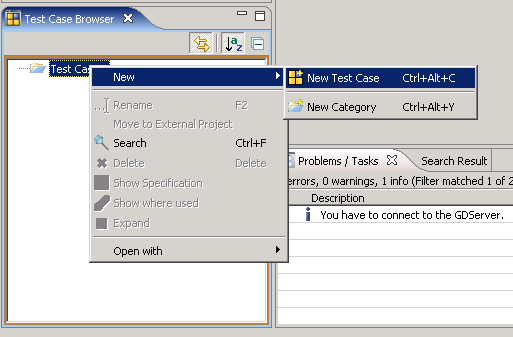
\includegraphics{Tutorials/PS/TutNewTestCase}
\caption{Creating a new Test Case}
\label{TutNewTestCase}
\end{center}
\end{figure}


 \item In the dialog which appears, name the \gdcase{}: \bxname{First Test}.
 \item Click \bxcaption{OK}. 
 \item You will see the \gdcase{} you just created as a node in the \gdtestcasebrowser{} (\bxfigref{TutCaseInBrowser}).

\begin{figure}[h]
\begin{center}
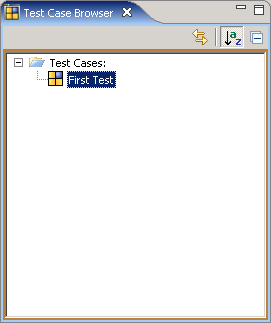
\includegraphics{Tutorials/PS/TutCaseInBrowser}
\caption{The \gdtestcasebrowser{}}
\label{TutCaseInBrowser}
\end{center}
\end{figure}
 
 \item Double-click on this node to open the \gdtestcaseeditor{}. 
 \item In this editor, right-click and select:\\ \bxmenu{Add}{New \gdstep{}}{}.
 \item You will see a dialog to specify a \gdstep{} (\bxfigref{TutFirstTestStep}). 

\begin{figure}[h]
\begin{center}
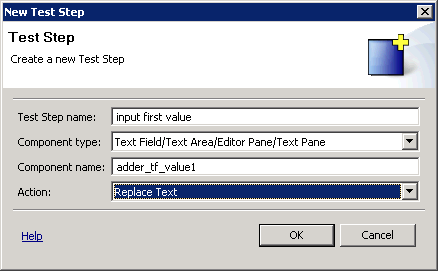
\includegraphics{Tutorials/PS/TutFirstTestStep}
\caption{The first \gdstep{}}
\label{TutFirstTestStep}
\end{center}
\end{figure}


 \item In this dialog:
\begin{itemize}
\item Enter \bxshell{input first value} as the name.
\item Select \bxname{Text Field/Text Area/Editor Pane/Text Pane} as the component type.
\item Enter \bxshell{adder\_tf\_value1} as the component name.
\item Select \bxname{Replace Text} as the action.
\item Press \bxcaption{OK}.
\end{itemize}
\item You will see this \gdstep{} appear underneath the \gdcase{} node in the \gdtestcaseeditor{}.
\item Select the \gdstep{} with a single-click from the editor. 
\item In the \gdpropview{}, double-click in the \bxname{parameter value} cell. 
\item Enter \bxshell{=V1} and press \bxkey{Enter}, then \bxcaption{save}. This is a reference for the parameter, whose value you will enter later. 
\item Create another new \gdstep{} by double-clicking on the \gdstep{} you just created in the \gdtestcaseeditor{}. 
\item The details for this \gdstep{} are as follows:
\begin{itemize}
\item Enter \bxshell{input second value} as the name.
\item Select \bxname{Text Field/Text Area/Editor Pane/Text Pane} as the component type.
\item Enter \bxshell{adder\_tf\_value2} as the component name.
\item Select \bxname{Replace Text} as the action.
\item Press \bxcaption{OK}.
\end{itemize}
\item Enter \bxshell{=V2} in the \bxname{parameter value} cell in the \gdpropview{} for this \gdstep{}, press \bxkey{Enter} and then click \bxcaption{save}.
\item Create two more \gdsteps{} as above and name them \bxshell{calculate} and 
\bxshell{verify} respectively. The \gdsteps{} should be specified as follows:

\begin{itemize} 
\item For the ''calculate'' \gdstep:
\\
\\
\begin{tabular}{|p{0.3\bxpicwidth}|p{0.3\bxpicwidth}|}\hline
 Component type:& Button/Check Box/Radio Button\\\hline
 Component name:& \bxshell{adder\_bt\_equals}\\\hline
 Action:& Click\\\hline
 Parameter -- Number of Clicks:& 1 (Default)\\\hline
Parameter -- Mouse Button:& 1 (Left -- Default) \\\hline
\end{tabular}
\\
\\
\item For the ''verify'' \gdstep{}:
\\
\\
\begin{tabular}{|p{0.3\bxpicwidth}|p{0.3\bxpicwidth}|}\hline
 Component type:& Text Field/Text Area/Editor Pane/Text Pane\\ \hline
 Component Name:& \bxshell{adder\_tf\_result}\\ \hline
 Action:& Check text\\ \hline
Parameter -- Value:& \bxshell{=RES}\\ \hline
\end{tabular}
\end{itemize}

\item You should now have a \gdtestcaseeditor{} containing 4 \gdsteps{}. 
\item Next to the \gdcase{} node in the editor, you should be able to see the three parameters you have referenced in this \gdcase{}: \bxcaption{V1; V2; RES} in square brackets (\bxfigref{firsttest}). 
\item Press the \bxcaption{save} button on the toolbar.
\begin{figure}[h]
\begin{center}
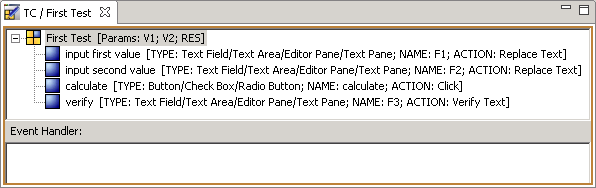
\includegraphics{GettingStarted/PS/firsttesteditor}
\caption{First Test \gdcase}
\label{firsttest}
\end{center}
\end{figure}
\end{enumerate}


